\chapter{Basis Transformationen }

Um die mathematischen Vorgehensweisen dieser Arbeit verständlicher zu machen, werden in den folgenden Kapiteln zunächst ein paar Grundlegende mathematische Operationen vorgestellt, welche das Grundgerüst der Stereokalibrierung und Szenenrekonstruktion bilden. Als aller erstes werden anhand praxisnaher Beispiele die Notwenidigkeit der Basis Transformation und damit einhergehend der Spezialfall einer Transformation von einem Koordinatensystem wie zum Beispiel \ensuremath{K_w = (O,\hat{e}_1,\hat{e}_2,\hat{e}_3)} in ein anderes Koordinatensystem  \ensuremath{K_c=(O_c, \hat{c}_1, \hat{c}_2, \hat{c}_3)} aufgezeigt. Anzumerken ist, dass grundlegend von orthogonalen Koordinatensystemen ausgegangen wird, sollte dies nicht der Fall sein, wird darauf nochmal explizit hingewiesen.\\

\section{Die Transformation von Koordinaten schließt die Transformation der Basis mit ein}

Es sei \textit{V} ein \textit{n}-Dimensionaler Vektorraum über einem Skalar beziehungsweise Körper \textit{K}. \textit{K} stellt in diesem Beispiel das Skalar \ensuremath{\mathbb{R}} dar, welches alle reelen Zahlen mit einschließt. Zur Veranschaulichung wird der Vektorraum \ensuremath{n=3} sprich \ensuremath{V^3} also ein 3-Dimesnionaler Raum gewählt, dessen Basis mit \ensuremath{\beta = [\vec{b}_1, \vec{b}_3, \vec{b}_3]} bezeichnet wird.\cite{Elements} ....  (FORTFÜHREN)


\section{Beispielhafte Vorführung von einem definierten Welt- zu einem synthetischen Kamerakoordinatensystem}

Anhand eines Beispiels wird die Transformation der Koordinaten noch genauer Veranschaulicht. Es soll kompakt in einer Symbolischen Schreibweise Punkte aus einem Weltkoordinatensystem  \ensuremath{K_w = (O,\hat{e}_1,\hat{e}_2,\hat{e}_3)} in ein Kamerakoordinatensystem \ensuremath{K_c=(O_c, \hat{c}_1, \hat{c}_2, \hat{c}_3)} überführt werden, welches eine Verschiebung und Rotation zum Weltkoordinatesystem aufweist. Beispielhaft wird dies in Abbildung 2.1. aufgezeigt.
 
	\begin{minipage}{\linewidth}
		\centering
		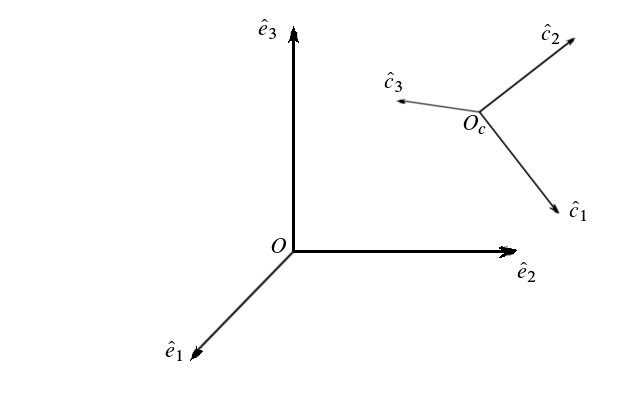
\includegraphics[width=1.\linewidth]{images/WeltKordSys.png}
		\captionof{figure}{Weltkoordinatensystem \ensuremath{K_w = (O,\hat{e}_1,\hat{e}_2,\hat{e}_3)} und Kamerakoordinatensystem \ensuremath{K_c=(O_c, \hat{c}_1, \hat{c}_2, \hat{c}_3)}}
	\end{minipage}\\ \\
	
	
	Zunächst wird wie im vorherigen Abschnitt beschrieben eine Koordinatisierung von Punkte im Weltkoordinatensystem vorgenommen. Ein Punkt \textit{P} wird dann wie folgt beschrieben.

	
	\begin{gather}
	P = O + p_1\hat{e}_1 + p_2\hat{e}_2 + p_3\hat{e}_3\\
	\leadsto(P)_{K_w} = (p_1,p_2,p_3)^T = \begin{pmatrix} p1 \\ p2 \\ p3 \end{pmatrix}
	\end{gather}
	
	Dieses Koordinatentupel wird dann zum Zweck der Einführung homogener Objekte projektiv Erweitert.
	
	\begin{gather}
	(P)_{K_w} = \begin{bmatrix} p_1 \\ p_2 \\ p_3 \\1 \end{bmatrix} = \left\{ k \begin{bmatrix} p_1\\p_2\\p_3\\1 \end{bmatrix} \in \mathbb{R} ^4 |  k \in \mathbb{R}\right\}
	\end{gather}
	
	Im Weltkoordinatensystem gilt des Weiteren:
	
	\begin{gather}
	\begin{bmatrix}\lambda p_1\\ \lambda p_2 \\ \lambda p_3 \\ 1 \end{bmatrix} = \begin{bmatrix}p_1 \\ p_2 \\ p_3 \\ 1\end{bmatrix} \text{für} \; \lambda \ne 0
	\end{gather}
	\pagebreak
	
	Ein Punkt bezüglich des Kamerakoordinatensystem wird im Vergleich wie folgt beschrieben.
	
	\begin{gather}
	K_c = (O_c, \hat{c}_1, \hat{c}_2, \hat{c}_3)\\
	_cP = O_c + _cp_1\hat{c}_1 + _cp_2\hat{c}_2 + _cp_3\hat{c}_3\\
	(P)_{K_c} = \begin{pmatrix}_cp_1 \\ _cp_2 \\ _cp_3\end{pmatrix}
	\end{gather}\\
	
	Zwischen diesen beiden Koordinatensystemen	 \ensuremath{K_w}  und \ensuremath{K_c} soll nun eine Beziehung hergestellt werden. Folgende Beziehungsgleichungen werden hierzu aufgestellt. 
	
	\begin{gather}
	O_c = O + o_{c,1}\hat{e}_1 + o_{c,2}\hat{e}_2 + o_{c,3}\hat{e}_3\\
	\hat{c}_1 = (c_1)_1\hat{e}_1 +  (c_1)_2\hat{e}_2 +  (c_1)_3\hat{e}_3\\
	\hat{c}_2 = (c_2)_1\hat{e}_1 +  (c_2)_2\hat{e}_2 +  (c_2)_3\hat{e}_3\\
	\hat{c}_3 = (c_3)_1\hat{e}_1 +  (c_3)_2\hat{e}_2 +  (c_3)_3\hat{e}_3
	\end{gather}
	
	Diese Beziehungsgleichungen können nun in Gleichung 2.1 eingesetzt werden.
	
	\begin{gather}
	\begin{split}
	P = O + (o_{c,1} + _cp_1(c_1)_1 + _cp_2(c_2)_1 + _cp_3(c_3)_1) \cdot \hat{e}_1 \\
	+ (o_{c,2} + _cp_1(c_1)_2 + _cp_2(c_2)_2 + _cp_3(c_3)_2) \cdot \hat{e}_2\\
	+ (o_{c,3} + _cp_1(c_1)_3 + _cp_2(c_2)_3 + _cp_3(c_3)_3) \cdot \hat{e}_3
	\end{split}
	\end{gather}
	
Hieraus lässt sich ein Gleichungssystem aufstellen und lösen in Form von:
	
	\begin{gather}
	\begin{split}
	p_1 = o_{c,1} + (o_{c,1} + _cp_1(c_1)_1 + _cp_2(c_2)_1 + _cp_3(c_3)_1) \\
	\leadsto \: p_1 - o_{c,1} =  (o_{c,1} + _cp_1(c_1)_1 + _cp_2(c_2)_1 + _cp_3(c_3)_1)
	\end{split}
	\end{gather}
	
Zu Bemerken ist, dass wenn \ensuremath{(P)_{K_c}} gegeben ist, erhält man auf diese Weise direkt \ensuremath{(P)_{K_w}}. Wenn jedoch \ensuremath{(P)_{K_w}} gegeben ist, so muss das LGS
	
	\begin{gather}
	\begin{bmatrix}(c_1)_1 & (c_2)_1 & (c_3)_1\\
	(c_1)_2 & (c_2)_2 & (c_3)_2\\
	(c_1)_3 & (c_2)_3 & (c_3)_3
	\end{bmatrix} 
	\begin{pmatrix}
	_cp_1\\ _cp_2 \\ _cp_3
	\end{pmatrix} = 
	\begin{pmatrix}
	p1- o_{c,1}\\
	p2- o_{c,2}\\
	p3- o_{c,3}
	\end{pmatrix}
	\end{gather}
	
	gelöst werden. Wenn \ensuremath{K_c} ein kartesisches Koordinatensystem ist, so ist die entstehende  koeffizientenmatrix \textit{M} orthogonal und es gilt \ensuremath{M_c^{-1} = M_c^T}. 
	\begin{gather}
	M_c^{T} = 
	\begin{bmatrix}(c_1)_1 & (c_1)_2 & (c_1)_3\\
	(c_2)_1 & (c_2)_2 & (c_2)_3\\
	(c_3)_1 & (c_3)_2 & (c_3)_3
	\end{bmatrix} \\
	\begin{split}
	\leadsto \: \begin{pmatrix}
	_cp_1\\
	_cp_2\\
	_cp_2 
	\end{pmatrix}
	= M_c^T 
	\begin{pmatrix}
	p_1 - o_{c,1}\\
	p_2 - o_{c,2}\\
	p_3 - o_{c,3}
	\end{pmatrix}
	\end{split} 
	\end{gather}
	
	Handelt es sich um kein kartesisches Koordinatensystem, so muss lediglich die Inverse \ensuremath{M_c^{-1}} anstatt \ensuremath{M_c^T} gebildet und wie gehabt verfahren werden.Im Folgenden wird nun noch einmal kompakt und in einer symbolischen Schreibweise die Transformation von Welt- in Kamerakoordinaten  festgehalten. Einmal wird wie bereits angefangen in Spaltenvektoren verfahren, einmal wird das selbe Verfahren mit Zeilenvektoren dargestellt. Grund hierfür ist, dass es beide Ansätze funktionieren und zum Beispiel das Programm \textit{MatLab} mit Spaltenvektoren verfährt, während im entstandenen Code dieser Arbeit mit Zeilenvektoren gearbeitet wurde. 
	Als Hilfestellung und zur Erinnerung gilt, dass \ensuremath{(\hat{c}_1,\hat{c}_2,\hat{c}_3)} durch Rotation \textit{R} aus \ensuremath{(\hat{e}_1,\hat{e}_2,\hat{e}_2)} entstanden ist. Da es sich aber in einem nicht-kartesischen Koordinatensystem nicht um eine orthogonale Drehmatrix handelt wird die Rotation \textit{R} in diesem Beispiel als Transformationsmatrix \textit{C} gekennzeichnet. Somit soll gezeigt werden, dass die Transformation unabhängig der Definition ihres ausgehenden Koordinatensystem allgemein formuliert werden kann. Es gilt für die Transformation von Welt- in Kamerakoordinaten ausgehend von Spaltenvektoren folgendes.
	
	\begin{gather}
	\begin{pmatrix}
	\hat{c}_1\\
	\hat{c}_2\\
	\hat{c}_3\\
	O_c
	\end{pmatrix} = 
	\begin{bmatrix}
	c_{11} & c_{21} & c_{31} & 0\\
	c_{12} & c_{22} & c_{32} & 0\\
	c_{13} & c_{23} & c_{33} & 0\\
	o_{c,1} & o_{c,2} & o_{c,3} & 1
	\end{bmatrix}
	\begin{pmatrix}
	\hat{e}_1\\
	\hat{e}_2\\
	\hat{e}_3\\
	O
	\end{pmatrix}\\
	C^T = C^{-1}= \begin{bmatrix}
	c_{11} & c_{12} & c_{13} \\
	c_{21} & c_{22} & c_{23} \\
	c_{31} & c_{32} & c_{33} \\
	\end{bmatrix}\\
	C = \begin{bmatrix}
	c_{11} & c_{21} & c_{31} \\
	c_{12} & c_{22} & c_{32} \\
	c_{13} & c_{23} & c_{33} \\
	\end{bmatrix}
	\end{gather}

Dementsprechend muss für die Rücktransformation von Kamera in Weltkoordinaten nur wieder die transformierte beziehungsweise die Inverse \ensuremath{C^T} gebildet werden. Des Weiteren muss der Verschiebungsvektor ebenfalls mit dieser Inversen Mulitpliziert werden, um diesen ebenfalls in das Zielkoordinatensystem zu überführen.
	
	
	\begin{gather}
	\leadsto \: \begin{pmatrix}
	\hat{e}_1\\
	\hat{e}_2\\
	\hat{e}_3\\
	O
	\end{pmatrix} = 
	\begin{bmatrix}
	c_{11} & c_{21} & c_{31} & 0\\
	c_{12} & c_{22} & c_{32} & 0\\
	c_{13} & c_{23} & c_{33} & 0\\
	&-(o_{c,1}, o_{c,2}, o_{c,3})C& & 1
	\end{bmatrix}
	\begin{pmatrix}
	\hat{c}_1\\
	\hat{c}_2\\
	\hat{c}_3\\
	O_c
	\end{pmatrix}
	\end{gather}
	
	
	
	
%	Die  Rücktransformation von Kamera- in Weltkoordinaten beinhaltet mit Spaltenvektoren dargestellt also folgendes:
%	
%	\begin{gather}
%	(a,b,c,1) 
%	\begin{bmatrix}
%	c_{11} & c_{12} & c_{13} & 0\\
%	c_{21} & c_{22} & c_{23} & 0\\
%	c_{31} & c_{32} & c_{33} & 0\\
%	o_{c,1} & o_{c,2} & o_{c,3} & 1
%	\end{bmatrix}
%	= (0,0,0,1)
%	\end{gather}
	
	Die Formel 2.21 zeigt die selbe Transformation nur werden die Koordinatensysteme als Zeilenvektoren dargestellt.

	\begin{gather}
	(\hat{c}_1, \hat{c}_2, \hat{c}_3, O_c) = (\hat{e}_1,\hat{e}_2, \hat{e}_3, O) \cdot
	\begin{bmatrix} 
	c_{11} & c_{21} & c_{31} & o_{c,1}\\
	c_{12} & c_{22} & c_{23} & o_{c,2}\\
	c_{13} & c_{32} & c_{33} & o_{c,3}\\
	0           &       0       &   0         & 1   
	\end{bmatrix}
	\end{gather}	
	
	Daraus folgt, dass für den Fall der Rücktransformation gilt:
	
	\begin{gather}
	\leadsto \: \begin{pmatrix}
	\hat{e}_1,\hat{e}_2,\hat{e}_3,O
	\end{pmatrix} = 
	\begin{bmatrix}
	c_{11} & c_{12} & c_{13} & \\
	c_{21} & c_{22} & c_{23} &  -\begin{pmatrix}
	o_{c,1}\\
	o_{c,2}\\
	o_{c,3}
	\end{pmatrix}C^T\\
	c_{31} & c_{32} & c_{33} & \\
	0&0&0 & 1
	\end{bmatrix}
	\begin{pmatrix}
	\hat{c}_1,\hat{c}_2,\hat{c}_3,O_c
	\end{pmatrix}
	\end{gather}
	
 Als Zwischenfazit lässt sich festhalten, dass sich die Matrix zur Beschreibung der Koordinatentransformation aus \textit{C} und einem Spalten- beziehungsweise Zeilenvektor der Form  \ensuremath{\vec{v}=\begin{pmatrix}
		o_{c,1}\\o_{c,2}\\o_{c,3}\\
	\end{pmatrix}} oder \ensuremath{\vec{v}=\begin{pmatrix}
	o_{c,1}&o_{c,2}&o_{c,3}\\
\end{pmatrix}} zusammensetzt.

\begin{gather}
		\begin{bmatrix}
	c_{11} & c_{21} & c_{31} & 0\\
	c_{12} & c_{22} & c_{32} & 0\\
	c_{13} & c_{23} & c_{33} & 0\\
	&-(o_{c,1}, o_{c,2}, o_{c,3})C& & 1
	\end{bmatrix}\\
		\begin{bmatrix}
	c_{11} & c_{21} & c_{31} & \\
	c_{12} & c_{22} & c_{32} & -\begin{pmatrix}
	o_{c,1}\\o_{c,2}\\ o_{c,3}
	\end{pmatrix}C\\
	c_{13} & c_{23} & c_{33} &\\
	0&0&0&1
	\end{bmatrix}
\end{gather}\\

Da im implementierten Code dieser Arbeit mit Zeilenvektoren gearbeitet wurde, wird nochmal in symbolischer Schreibweise sämtliche Schritte der Koordinatentransformation im folgenden zusammengefasst. 

\begin{gather}
\begin{pmatrix}
&&K&&
\end{pmatrix}
\begin{bmatrix}
\begin{pmatrix}\\c_1\\\\ \end{pmatrix}_k & \begin{pmatrix}\\c_2\\\\ \end{pmatrix}_k & \begin{pmatrix}\\c_3\\\\ \end{pmatrix}_k & \begin{pmatrix}\\O_c\\\\ \end{pmatrix}_k\\
0&0&0&1
\end{bmatrix} = \begin{pmatrix}
&&K_c&&
\end{pmatrix}\\
\leadsto \: 
\begin{pmatrix}
\hat{e}_1,\hat{e}_2,\hat{e}_3,O
\end{pmatrix} = 
\begin{bmatrix}
&  &  & \\
&  C&  &\vec{v} \\ 
&  &  & \\
0&0&0 & 1
\end{bmatrix}
\begin{pmatrix}
\hat{c}_1,\hat{c}_2,\hat{c}_3,O_c
\end{pmatrix}
\end{gather}
%\ensuremath{\rightarrow \text{Matrix einer affinen Transformation}

Sei im Weltkoordinatensystem ein Punkt \ensuremath{P} = \ensuremath{\begin{pmatrix}
		\hat{e}_1,\hat{e}_2,\hat{e}_3,O
	\end{pmatrix} 
	\begin{pmatrix}
		p1\\p2\\p3\\1
	\end{pmatrix} = 
	\begin{pmatrix}
		\hat{c}_1,\hat{c}_2,\hat{c}_3,O_c
	\end{pmatrix} 
	\begin{pmatrix}
		_cp_1\\
		_cp_2\\
		_cp_2\\
		1 
\end{pmatrix}} im Kamerakoordinatensystem, so liefert die Transformation von Welt- in  Kamerakoordinatensystem folgendes

\begin{gather}
\begin{pmatrix}
\hat{c}_1,\hat{c}_2,\hat{c}_3,O_c
\end{pmatrix}
\begin{bmatrix}
&  &  & \\
&  C&  &\vec{v} \\ 
&  &  & \\
0&0&0 & 1
\end{bmatrix}
\begin{pmatrix}
_cp_1\\
_cp_2\\
_cp_2\\
1 
\end{pmatrix} =
\begin{pmatrix}
\hat{e}_1,\hat{e}_2,\hat{e}_3,O
\end{pmatrix}
\begin{pmatrix}
p1\\p2\\p3\\1
\end{pmatrix}
\end{gather}

Aus der Eindeutigkeit der Koordinatendarstellung folgt:

\begin{gather}
\begin{bmatrix}
&  &  & \\
&  C&  &\vec{v} \\ 
&  &  & \\
0&0&0 & 1
\end{bmatrix}
\begin{pmatrix}
\begin{pmatrix}
\\
P_{kc}\\
\\
\end{pmatrix}_k\\
1
\end{pmatrix}
=
\begin{pmatrix}
\begin{pmatrix}
\\
P_k\\
\\
\end{pmatrix}_k\\
1
\end{pmatrix}
\end{gather}\\


Und umgekehrt resultiert aus der Transformation von Kamera- in Weltkoordinaten wie bereits gezeigt:

\begin{gather}
\leadsto \: \begin{pmatrix}
\hat{e}_1,\hat{e}_2,\hat{e}_3,O
\end{pmatrix} = 
\begin{bmatrix}
c_{11} & c_{12} & c_{13} & \\
c_{21} & c_{22} & c_{23} &  -\begin{pmatrix}
o_{c,1}\\
o_{c,2}\\
o_{c,3}
\end{pmatrix}C^T\\
c_{31} & c_{32} & c_{33} & \\
0&0&0 & 1
\end{bmatrix}
\begin{pmatrix}
\hat{c}_1,\hat{c}_2,\hat{c}_3,O_c
\end{pmatrix}
\end{gather}

%Die Form der Rücktransformation von Kamera- in Weltkoordinaten beinhaltet folgendes:
%
%\begin{gather}
%(a,b,c,1) 
%\begin{bmatrix}
%c_{11} & c_{21} & c_{31} & o_{c,1}\\
%c_{12} & c_{22} & c_{32} & o_{c,2}\\
%c_{13} & c_{23} & c_{33} & o_{c,3}\\
%0 & 0 & 0 & 1
%\end{bmatrix}
%= (0,0,0,1)
%\end{gather}
Zur Probe kann folgende Gleichung aufgestellt und auf ihren Wahrheitswert geprüft werden 

\begin{gather}
\begin{bmatrix}
& & & \\
& C^T & & -\begin{pmatrix}
o_{c,1}\\
o_{c,2}\\
o_{c,3}
\end{pmatrix}C^T \\
& & & \\
0&0 &0 & 1
\end{bmatrix}
\begin{bmatrix}
& & & o_{c,1}\\
& C & & o_{c,2}\\
& & &o_{c,3} \\
0&0 &0 & 1
\end{bmatrix}
=
\begin{bmatrix}
1&0 &0 & 0\\
0& 1 &0 & 0\\
0& 0& 1& 0\\
0& 0 &0 & 1
\end{bmatrix}
\end{gather}\\

In allgemeiner symbolischer Form gilt also\\

\begin{gather}
\begin{pmatrix}
\begin{pmatrix}
\\
P_{kc}\\
\\
\end{pmatrix}_k\\
1
\end{pmatrix}
=
\begin{bmatrix}
&  &  & \\
&  C&  &\vec{v} \\ 
&  &  & \\
0&0&0 & 1
\end{bmatrix}^{-1}
\begin{pmatrix}
\begin{pmatrix}
\\
P_k\\
\\
\end{pmatrix}_k\\
1
\end{pmatrix}
=
\begin{bmatrix}
&  &  & \\
&  C^{-1}&  &-\begin{pmatrix}
\\
C^{-1})\\
\\
\end{pmatrix}\vec{v} \\ 
&  &  & \\
0&0&0 & 1
\end{bmatrix}
\end{gather}\\

Und falls

\begin{gather}
\begin{pmatrix}
\hat{c}_1,\hat{c}_2,\hat{c}_3,O
\end{pmatrix}
=
\begin{pmatrix}
\hat{e}_1,\hat{e}_2,\hat{e}_3,O
\end{pmatrix}
\begin{bmatrix}
&  &  & \\
&  C&  &\vec{v} \\ 
&  &  & \\
0&0&0 & 1
\end{bmatrix}
\end{gather}
gilt, so ergibt sich
\begin{gather}
\begin{pmatrix}
_cp_1\\
_cp_2\\
_cp_3\\
1
\end{pmatrix}
=
\begin{bmatrix}
&  &  & \\
&  C^{-1}&  &-C^{-1}(O_c)_K \\ 
&  &  & \\
0&0&0 & 1
\end{bmatrix}
\begin{pmatrix}
p_1\\
p_2\\
p_3\\
1
\end{pmatrix}
\end{gather}


Somit wurde die symbolischen Transformationsformeln für die Objekte \ensuremath{(O,\hat{e}_1,\hat{e}_2,\hat{e}_3)} der Koordinatensysteme festgehalten. Jetzt zurück zur Transformation der Koordinatentupel. Aus Gleichung 2,14 folgt:\\


\begin{gather}
C \,
\begin{pmatrix}
_cp_1\\
_cp_2\\
_cp_3
\end{pmatrix}
=
\begin{pmatrix}
p_1 - o_{c,1}\\
p_2 - o_{c,2}\\
p_3 - o_{c,3}
\end{pmatrix} | C^T\\
_cp := \begin{pmatrix}
_cp_1\\
_cp_2\\
_cp_3
\end{pmatrix}
= C^T 
\begin{pmatrix}
p_1\\
p_2\\
p_3
\end{pmatrix}
-
C^T 
\begin{pmatrix}
o_{c,1}\\
o_{c,2}\\
o_{c,3} 
\end{pmatrix} \mid \text{projektive Erweiterung}\\
\begin{bmatrix}
_cp\\
1
\end{bmatrix}
=
\begin{bmatrix}
& & & \\
& C^T & & -{C^T}_{o_c}\\
& & & \\
0&0 &0 & 1
\end{bmatrix}
\begin{bmatrix}
P\\
1
\end{bmatrix}
\end{gather}
\pagebreak

Und umgekehrt gilt

\begin{gather}
\begin{bmatrix}
P\\
1
\end{bmatrix}
=
\begin{bmatrix}
& & & \\
& C & & O_c\\
& & & \\
0&0 &0 & 1
\end{bmatrix}
=
\begin{bmatrix}
_cp\\
1
\end{bmatrix}
\end{gather}

Daraus lässt sich also die folgende Aussage ableiten. 
\begin{gather}
\begin{pmatrix}
p_1\\
p_2\\
p_3\\
1
\end{pmatrix}
=
\begin{bmatrix}
\begin{pmatrix}\\c_1\\\\ \end{pmatrix}_k & \begin{pmatrix}\\c_2\\\\ \end{pmatrix}_k & \begin{pmatrix}\\c_3\\\\ \end{pmatrix}_k & O_c\\
0&0&0&1
\end{bmatrix}
\begin{bmatrix}
_cp_1\\
_cp_2\\
_cp_3\\
1
\end{bmatrix}
\end{gather}

\begin{gather}
\begin{pmatrix}
p_1\\
p_2\\
p_3\\
1
\end{pmatrix}
=
\begin{bmatrix}
_cp_1\begin{pmatrix}\\c_1\\0\\\\ \end{pmatrix} + _cp_2\begin{pmatrix}\\c_2\\0\\\\ \end{pmatrix} + _cp_3\begin{pmatrix}\\c_3\\0\\\\ \end{pmatrix} + \begin{pmatrix}\\O_c\\1\\\\ \end{pmatrix}
\end{bmatrix}
\end{gather}
	
\section{Übersicht über die benötigten Koordinatensysteme und Transformationen für die Stereobildanalyse}
	
Nachdem die mathematische Grundlage der Basis - beziehungsweise Koordinatentransformation erläutert wurde, muss diese nun für den Fall der Stereokalibrierung und 3D-Szenerekonstruktion entsprechend erweitert werden. Es müssen folgende Überlegungen gemacht werden. Zum einen muss geklärt werden, wie viele Transformationen nötig sind, um von einem 3D-Objekt in Weltkoordinaten auf ein projiziertes 2D-Bild dieses Objektes auf dem Sensor zu kommen. Zum anderen müssen die entsprechenden Basen dieser Koordinatensysteme definiert werden.

\section{Aubau der Koordinatenssysteme}
		
Insgesamt werden für die Stereoanalyse fünf verschiedene Koordinatensysteme Definiert. Das Weltkoordinatensysten, die Kamerakooridnatensysteme, Das Bildebenenkoordinatensystem und das Sensorkoordinatensystem. Grundlegend wird erst einmal festgelegt, welche Orientierungen die Koordinatensysteme haben sollen. Die Arbeit und auch die entstanden Algorithmen basieren auf rechtsdrehenden Systemen. Die Möglichkeit linksdrehende Systeme zu benutzen sind aus dem entstandenen Algorithmus nicht ausgeschlossen, jedoch ist es für die spätere Deutung und Interpretation der Resultate wichtig im Vorhinein definiert zu haben, wie die Orientierung der einzelnen Koordinatensysteme ist. Das Weltkoordinatensystem wird mit \ensuremath{K_w=(\hat{e}_1,\hat{e}_2,\hat{e}_3,O )} definiert, um die Notation des Beispiels im vorherigen Abschnitts einzuhalten und Verwirrung zu vermeiden. Des Weiteren wird festgehalten, dass das Weltkoordinatensystem gleich dem Koordinatensystem von einer der beiden Kameras entspricht. Die Bildebene ist gleich einer Ebene im 3D-Raum und wird mit \ensuremath{E} bezeichnet. Das Projektionszentrum auf der Bildebene bekommt die Notation \ensuremath{Z} zugeordnet. Die Kamerakoordinatensysteme sind wie das Weltkoordinatensystem kartesische rechtsdrehende Systeme. Für die Erklärung der Projektionen reicht es wenn wir zunächst den Weg von einem Objekt im 3D-Raum auf sein projiziertes Bild in einer der beiden Kameras genauer betrachten. Wie im Abschnitt zuvor wird dieses Kamerakoordinatensystem mit \ensuremath{K_c= (\hat{c}_1,\hat{c}_2,\hat{c}_3,O_c)} definiert. Des Weiteren soll gelten, dass \ensuremath{O_c = Z}, sprich der Ursprung des Kamerakoordinatensystems Deckungsgleich mit dem Projektionszentrum auf der Bildebene ist und somit auch \ensuremath{ <\hat{c}_1,\hat{c}_2> + P = E}. \ensuremath{P} bezeichent hier den Hauptpunkt der Bildebene.. Für die Wahl der Kamerakoordinatenachsen wird folgendes Schema verfolgt: \ensuremath{\hat{c}_1 \cdot \hat{n} = 0}, \ensuremath{\hat{c}_2 \cdot \hat{n} = 0}, \ensuremath{\hat{c}_3  = \pm\;\hat{n}}.  Die Bildebene selbst bekommt auch ein eigenes Koordinatensystem zugewiesen, welches sich aber nicht mehr auf einen 3D-Raum sondern auf die 2D-Ebene bezieht. Es soll \ensuremath{K_b = (\hat{b}_1,\hat{b}_2,O_b)} mit \ensuremath{O_b = P}, \ensuremath{\hat{b}_1 = \hat{c}_1}, \ensuremath{\hat{b}_2 = \hat{c}_2} gelten.  Formuliert man die Bildebene in Hess'scher Normalform so gilt \ensuremath{E: \hat{n} \cdot (\vec{x} - \vec{p}) = 0}. Als letztes kommt noch das Sensorkoordinatensystem mit  \ensuremath{K_s = (\vec{u}, \vec{v}, O_s)}. Dieses Koordinatensystem ist an die Geometrie der Pixel und des Sensors angepasst und daher muss es sich nicht unbedingt um ein kartesisches Koordinatensystem handeln.\\

Nachdem die einzelnen Koordinatensysteme definiert sind, soll zunächst wieder symbolisch die Projektion eines Objekts aus dem 3D-Raum auf den 2D-Sensor durchgerechnet werden.Für die Transformation der Weltkoordinatenachsen in Kamerakoordinatenachsen gilt: \ensuremath{C\hat{e}_i = \hat{c}_i}, wobei \ensuremath{C} eine 3x3-Rotationsmatrix darstellt. Es kann also wie bereits bekannt eine Matrix \ensuremath{M} aufgestellt werden, welche das Weltkoordinatensystem in das Kamerakoordinatensystem überführt. Der Verschiebevektor \ensuremath{\vec{v}} besteht aus den Koordinaten des Projektionszentrums \textit{Z}. Es gilt also \ensuremath{\vec{v} = Z \leadsto \vec{v} = \begin{pmatrix}
		z_1\\z_2\\z_3
\end{pmatrix}}.

\begin{gather} 		
(\hat{e}_1,\hat{e}_2,\hat{e}_3)[D] =(\hat{c}_1, \hat{c}_2, \hat{c}_3) \leadsto \hat{c}_1 = D_{11}\hat{e}_1 + D_{21} \hat{e}_2 + D_{31}\hat{e}_3\\	
\begin{bmatrix}
\\D\\\\
\end{bmatrix}
=	\begin{bmatrix}
\begin{pmatrix}
\\
\hat{c}_1\\
\\
\end{pmatrix}_K
\begin{pmatrix}
\\
\hat{c}_2\\
\\
\end{pmatrix}_K
\begin{pmatrix}
\\
\hat{c}_3\\
\\
\end{pmatrix}_K
\end{bmatrix}\\
(\hat{c}_1, \hat{c}_2, \hat{c}_3,O_c)=(\hat{e}_1,\hat{e}_2,\hat{e}_3,O) \cdot
\begin{bmatrix}
&  &  &z_1 \\
&  [D]&  &z_2 \\ 
&  &  &z_3 \\
0&0&0 & 1
\end{bmatrix}	
\end{gather}

des weiteren müssen die Transformierten Koordinaten noch mit einer entsprechenden Projektion auf die Kamera projiziert werden. Hierzu muss eine Projektionsmatrix der Form

	\begin{gather}
\leftidx{_{K_{c_1}}}{\begin{bmatrix}
	\pi
	\end{bmatrix}}{_{K_{c_2}}} 
= 
\begin{pmatrix}
\zeta&0&0&0\\
0&\zeta&0&0\\
0&0&\zeta&0\\
0&0&1&0
\end{pmatrix}
\end{gather}

aufgestellt werden. Zur Probe dient 


\begin{gather}
\begin{bmatrix}
X\\Y\\Z\\1
\end{bmatrix} \mapsto
\begin{pmatrix}
\zeta X\\ \zeta Y\\ \zeta Z \\ Z
\end{pmatrix}
=
\begin{pmatrix}
\zeta \frac{X}{Z}\\ \zeta \frac{Y}{Z}\\ \zeta  \\ 1
\end{pmatrix}
\end{gather}


Im folgenden wird die Bedeutung hinter $\zeta$ hergeleitet. Einmal in Bezug der Projektion von Kamera- in Kamerakoordinaten. Danach in Bezug auf die Projektion von Kamera- in Bildebenenkoordinaten. In der Literatur  wird $\zeta$ meist mit $f$ für \textit{focal length} dargestellt und die Bildebene auch \textit{Focal plane} genannt \cite{HZ}. Hierzu wird später bei der Projektion auf die 2D Bildebene noch genaueres erläutert.

	\begin{minipage}{\linewidth}
	\centering
	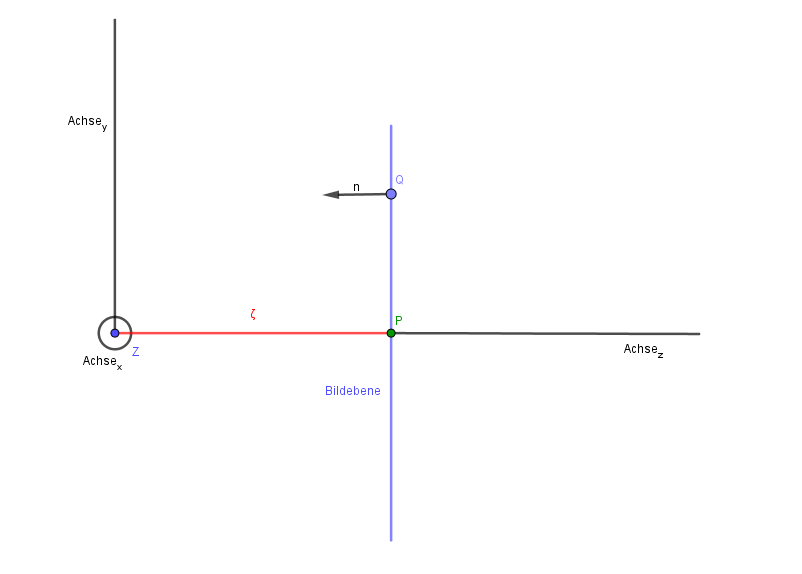
\includegraphics[width=1.\linewidth]{images/ZetaHerleitung.png}
	\captionof{figure}{In blau ist die Bildebene dargestellt auf ihr befinden sich die Punkte $Q$ und $P$. $Z$ liegt nicht auf der Ebene, Das Projetionszenter liegt hinter der Bildebene und somit auch hinter dem Sensor. $n$ ist die Normale der Bildebene}
\end{minipage}\\

Wie in Abbildung 2.2 ersichtlich kann für die Findung von $\zeta$, welche den Abstand des Projektionszentrums zur Bildebene beschreibt, folgende Gleichung aufgestellt werden
		
		\begin{gather}
		\vec{p}+|\vec{QZ} \cdot \vec{n}|\vec{n} = \vec{Z}
		\end{gather}
		
		Q ist ein beliebiger Punkt auf der Ebene. Setze
		\begin{gather}
		\vec{QZ} \cdot \hat{n} = \zeta\\
		\vec{p}= \vec{Z}\zeta \hat{n}
		\end{gather}
		
		Wählt man nun  $\hat{c}_3 = \hat{n}$ so kann daraus geschlossen werden, dass $\vec{p} = \vec{Z} - \zeta \hat{n}$. Für die folgende Projektion der Koordinaten im 3D-Kamerakoordinatensystems auf das 2D-Bildebenenkoordinatensystem muss eine Projektionsmatrix der Form		
		
		\begin{gather}
		\leftidx{_{K_{b}}}{\begin{bmatrix}
			\pi
			\end{bmatrix}}{_{K_{c}}} 
		= 
		\begin{pmatrix}
		\zeta&0&0&0\\
		0&\zeta&0&0\\
		0&0&1&0\\
		\end{pmatrix}
		\end{gather}
		 aufgestellt werden. Es gilt allgemein dass $O_B = Z - \zeta \hat{n} = \vec{p}, \; \hat{b}_1 = \hat{c}_1, \; \hat{b}_2 = \hat{c}_2$ ist. Zur Probe ob die Projektionsmatrix stimmt wird folgendes gerechnet.
		\begin{gather}
\begin{bmatrix}
X\\Y\\Z\\1
\end{bmatrix} \mapsto
\begin{pmatrix}
\zeta X\\ \zeta Y\\ Z
\end{pmatrix}
=
\begin{bmatrix}
\zeta&0&0&0\\
0&\zeta&0&0\\
0&0&1&0
\end{bmatrix}
\cdot
\begin{bmatrix}
X\\Y\\Z\\1
\end{bmatrix}
=
\begin{pmatrix}
\zeta \frac{X}{Z}\\ \zeta \frac{Y}{Z}\\1
\end{pmatrix}
\end{gather}

		Der Übergang von Kamerakoordinaten in Bildkoordinaten wird im folgenden nochmal bezogen auf das in dieser Arbeit definierte Modell beschrieben. 
		
		\begin{gather}
		(\hat{b}_1, \hat{b}_2, O_B) = (\hat{c}_1,\hat{c}_2,\hat{c}_3,O_c) \cdot 
		\begin{bmatrix}
		1&0&0\\
		0&1&0\\
		0&0&\zeta\\
		0&0&1
		\end{bmatrix}
		\end{gather}\\
		
		Sei $(X)_B = \begin{pmatrix}
		x_1\\x_2\\1
		\end{pmatrix}$
		
		\begin{gather}
		\leadsto (x)_c = \begin{pmatrix}
		x_1\\x_2\\\zeta\\1
		\end{pmatrix} 
		=
		\begin{bmatrix}
		1&0&0\\
		0&1&0\\
		0&0&\zeta\\
		0&0&1
		\end{bmatrix} \cdot
		\begin{pmatrix}
		x_1\\x_2\\1
		\end{pmatrix}
		\end{gather}\\
		
		Für die Umkehrung muss hier mit der Pseudoinversen gearbeitet werden. Um die Projektionsmatrix welche die Bildebenenkoordinaten wieder in Kamerakoordinaten projiziert zu finden muss folgende Rechenoperation durchgeführt werden. 
		
		\begin{gather}
		\begin{pmatrix}
		x_1\\x_2\\1
		\end{pmatrix} 
		=
		\begin{bmatrix}
		1&0&0&0\\
		0&1&0&0\\
		0&0&0&1\\
		\end{bmatrix} \cdot
		\begin{pmatrix}
		x_1\\x_2\\\zeta\\1
		\end{pmatrix}\\
		\leadsto 	
		\leftidx{_{K_{c}}}{\begin{bmatrix}
			\pi
			\end{bmatrix}}{_{K_{b}}} 
		= 	\begin{bmatrix}
		1&0&0&0\\
		0&1&0&0\\
		0&0&0&1\\
		\end{bmatrix} \cdot
		\begin{pmatrix}
		\zeta&0&0&0\\
		0&\zeta&0&0\\
		0&0&\zeta&0\\
		0&0&1&0
		\end{pmatrix} 
		=
		\begin{pmatrix}
		\zeta&0&0&0\\
		0&\zeta&0&0\\
		0&0&1&0\\
		\end{pmatrix}
		\end{gather}\\
		
		Um die Projektionsmatrix allgemeiner zu formulieren und die Bedeutung und hinter $\zeta$ und dessen Zusammenhang mit dem in der Literatur benutzten $f$ genauer zu erläutern, wird die Projektionsmatrix der Photogrammetrie in Bezug auf ein Lochkameramodell\cite{HZ} hier noch einmal genauer betrachtet und mit dem hergeleiteten Modell verglichen. Nehmen wir an es gilt $\zeta = f$, dann gilt für die Projektion von Punkten das selbe wie in Gleichung 2.49 nur mit $f$ statt $\zeta$. 
		
				\begin{gather}
		\begin{bmatrix}
		X\\Y\\Z\\1
		\end{bmatrix} \mapsto
		\begin{pmatrix}
		\zeta X\\ \zeta Y\\ Z
		\end{pmatrix}
		=
		\begin{bmatrix}
		\zeta&0&0&0\\
		0&\zeta&0&0\\
		0&0&1&0
		\end{bmatrix}
		\cdot
		\begin{bmatrix}
		X\\Y\\Z\\1
		\end{bmatrix}
		=
		\begin{pmatrix}
		\zeta \frac{X}{Z}\\ \zeta \frac{Y}{Z}\\1
		\end{pmatrix}\\
	\leadsto
		\begin{bmatrix}
		X\\Y\\Z\\1
		\end{bmatrix} \mapsto
		\begin{pmatrix}
		f X\\ f Y\\ Z
		\end{pmatrix}
		=
		\begin{bmatrix}
		f&0&0&0\\
		0&f&0&0\\
		0&0&1&0
		\end{bmatrix}
		\cdot
		\begin{bmatrix}
		X\\Y\\Z\\1
		\end{bmatrix}
		=
		\begin{pmatrix}
		f \frac{X}{Z}\\ f \frac{Y}{Z}\\1
		\end{pmatrix}
		\end{gather}
		
		Zum Vergleich dient die Definition im Buch von \textit{Hartley \& Zisserman}\cite{HZ}, welche der selbst hergeleiteten entspricht.
		
		
					\begin{gather}
		\begin{bmatrix}
		X\\Y\\Z\\1
		\end{bmatrix} \mapsto
		\begin{pmatrix}
		f X\\ f Y\\ Z
		\end{pmatrix}
		=
		\begin{bmatrix}
		f&0&0&0\\
		0&f&0&0\\
		0&0&1&0
		\end{bmatrix}
		\cdot
		\begin{bmatrix}
		X\\Y\\Z\\1
		\end{bmatrix}
		\end{gather}		
		
		
		Die komplette Projektionsmatrix $K$ lautet in der Literatur wie folgt\cite{HZ}
		
		\begin{gather}
		K=\begin{bmatrix}
		\alpha_x&s&x_{0}\\
		0&\alpha_y&y_{0}\\
		0&0&1
		\end{bmatrix}
		\end{gather}
		
		Um zu verstehen was die Bedeutung hinter $\alpha_x$ und $\alpha_y$ ist, sollte zunächst noch geklärt werden, dass im hergeleiteten Ansatz dieser Arbeit davon ausgegangen wird, dass die \textit{focal length} $\zeta$ beziehungsweise $f$ in $x$- sowie in $y$-Richtung einheitlich ist. Dies ist jedoch nicht immer der Fall. Bei den bekannten und viel genutzten CCD-Kamerachips trifft es zu, dass die Bildkoordinaten und Sensorkoordinaten einheitliche Quadrate bilden,Jedoch gibt es ebenfalls Chips, bei denen es nicht-quadratische Pixel gibt\cite{HZ}. Wird so ein Chip genutzt, so sind die Werte für $f$ nicht mehr identisch, weshalb beide $f$ meist einen Index besitzen und es steht dann jeweils $f_x$ und $f_y$ in der Matrix. Dies soll aufzeigen, dass es sich auch wenn die Werte identisch sein sollte, es sich trotzdem um zwei Verschiedene \textit{focal length}- Einheiten handelt. Sind die Pixel nicht quadratisch, wird auf die Werte $f_x$ und $f_y$ jeweils eine Skalierung $m_x$ und $m_y$ drauf multipliziert so dass  $\alpha_x = f_x \cdot m_x$ und $\alpha_y = f_y \cdot m_y$ entspricht.\cite{HZ}. $x_{0}$ und $y_{0}$ bilden einen Verschiebungsvektor. Sie beinhalten die Definition wo sich der Hauptpunkt auf der Bildebene befindet. $x_{0}$ und $y_{0}$ sind definiert als $x_{0} = p_x \cdot m_x$ und $x_{0} = p_y \cdot m_y$. Die Die Variable $s$ wird dem sogenannten \textit{skew-Faktor} zugeordnet, welcher nur dann zum Einsatz kommt, sollte die optische Achse nicht orthogonal auf den Chip auftreffen. Sprich wenn der Chip geneigt in der Kamera montiert wurde\cite{HZ}.Die komplette Kameramatrix $P=KM=K[C|t]$ beziehungsweise wie sie in der Literatur zitiert wird $P=K[R|t]$\cite{HZ} besteht aus der Matrixmultiplikation der hergeleiteten Transformationsmatrix $M$ welche die externen Kamerparameter repräsentiert und der Projektionsmatrix $K$, welche die internen Kameraparameter repräsentiert. $P$ beinhaltet also sowohl die internen als auch die externen Kameraparameter. \\
		
		Zuletzt folgt nun noch die Transformation der Bildebenenkoordinaten in die Sensorkoordinaten, welches mit $K_s = (\vec{u},\vec{v}, O_s)$ definiert ist. $\vec{u}$ und $\vec{v}$ beinhalten wie bereits erwähnt die Information über die Geometrische Beschaffung der Pixel und muss sich dem entsprechend nicht zwangsläufig ein kartesisches Koordinatensystem sein. Das Koordinatensystem wird also folgendermaßen definiert
		
		\begin{gather}
		\vec{u} = u_1 \hat{b}_1 + u_2 \hat{b}_2\\
		\vec{v} = v_1 \hat{b}_1 + v_2 \hat{b}_2\\
		O_S = O_B +p_1 \hat{b}_1 + p_2 \hat{b}_2\\
		\begin{pmatrix}
		\vec{u}, \vec{v}, O_S
		\end{pmatrix}		
		=
		\begin{pmatrix}
		\hat{b}_1, \hat{b}_2, O_B 
		\end{pmatrix}\cdot	
		\begin{bmatrix}
		u_1&v_1&p_1\\u_2&v_2&p_2\\0&0&1\\
		\end{bmatrix}
		\end{gather}
		
		Anhand eines Beispiels wird nun symbolisch durchgerechnet was das für die Bildebenenkoordinaten bedeutet. 
		
		Es sei $(X)_S=\begin{pmatrix}
		a\\b\\1
		\end{pmatrix}$
		
		\begin{gather}
		\leadsto x = a \vec{u} + b \vec{v} + O_S\\
		= a (u_1 \hat{b}_1 + u_2 \hat{b}_2) +b(v_1 b_1 + v_2 b_2) + O_B + p_1 b_1\\
		\mapsto (X)_B = \begin{bmatrix}
		p_1 + a v_1 + b v_1\\
		p_2 + a u_2 + b u_2
		\end{bmatrix}\\
		(X)_S =
		\begin{bmatrix}
		&  & \\
		&\begin{bmatrix}
		u_1& v_1\\
		u_2& v_2
		\end{bmatrix}^{-1}  & -M^{-1}\begin{pmatrix}
		p_1\\p_2
		\end{pmatrix} \\ 
		&  & \\
		0&0 & 1
		\end{bmatrix}
		\cdot
		\begin{bmatrix}
		&&\\
		&X&\\
		&&
		\end{bmatrix}_B	
		\end{gather}\\
		
		 $	\leftidx{_{K_{s}}}{\begin{bmatrix}
			\pi
			\end{bmatrix}}{_{K_{c}}} $ wird also dementsprechend wie folgt dargestellt\\
		
		\begin{gather}	\leftidx{_{K_{s}}}{\begin{bmatrix}
			\pi
			\end{bmatrix}}{_{K_{c}}} 
		=
		\begin{bmatrix}
		&&\\
		&M^{-1}& -M\begin{pmatrix}p_1\\p_2\end{pmatrix}^{-1}\\
		&&\\
		0&0&1
		\end{bmatrix}
		\cdot
		\begin{bmatrix}
		-\zeta&0&0&0\\
		0&-\zeta&0&0\\
		0&0&1&0
		\end{bmatrix}
		=
		\begin{bmatrix}
		&&&0\\
		&-\zeta M^{-1}& -M\begin{pmatrix}p_1\\p_2\end{pmatrix}^{-1}&0\\
		&&&\\
		0&0&1&0
		\end{bmatrix}
		\end{gather}
		
		Zur Verdeutlichung folgen nun noch zwei Beispiele. Es werden $\vec{u}$ und $\vec{v}$, sowie $p_1$ und $p_2$ mit Werten versehen. $p$ entspricht symbolisch einem \textit{Pixelpitch}-Wert. Mit \textit{Pixelpitch} wird der direkte Abstand der Pixel auf Bildsensoren zwischen Pixelmitte zu Pixelmitte bezeichnet. Wir definieren also\\
		
		$\vec{u} = 1pb_1 $\\
		$\vec{v} = 2pb_2 $\\
		$ p_1 = 15, p_2 = 20$\\
		
		Für die Projektionsmatrix ergibt sich dann
		
		\begin{gather}
		O_S = O_B - \vec{u} - \vec{v} \leadsto O_S = O_B -15 b_1 - 20 b_2\\	
		M= 
		\begin{bmatrix}
		1&0\\
		0&2
		\end{bmatrix}
		\leadsto
		M^{-1}=\begin{bmatrix}
		\frac{1}{p}&0\\
		0&\frac{1}{2p}
		\end{bmatrix}\\
		[\pi] =
		\begin{bmatrix}
		\frac{-\zeta}{p}&0&15&0\\
		0&\frac{-\zeta}{p}&20&0\\
		0&0&1&0
		\end{bmatrix}
		\end{gather}\\
		
	  Zum Nachvollziehen gibt es hier nochmal ein anderes Beispiel.\\
		
		$\vec{v} = 1pb_1+2pb_2$\\
		$\vec{u} = 1pb_1$\\
		$ p_1 = 10, p_2 = 5$\\
		
		\begin{gather}
		M=\begin{bmatrix}
		1&1\\
		0&2
		\end{bmatrix} \leadsto 
		M^{-1} =
		\begin{bmatrix}
		1&-\frac{1}{2}\\
		0&\frac{1}{2}
		\end{bmatrix} \\
		\leftidx{_{K_{s}}}{\begin{bmatrix}
			\pi
			\end{bmatrix}}{_{K_{c}}}
		= 
		\begin{bmatrix}
		\frac{-\zeta}{p}&\frac{-\zeta}{2p}&10&0\\
		0&\frac{-\zeta}{p}&5&0\\
		0&0&1&0
		\end{bmatrix}\\
		= [K|0]
		\end{gather}
		
		Zusammengefasst wird hier noch einmal die symbolische Darstellung von $	\leftidx{_{K_{s}}}{\begin{bmatrix}
			\pi
			\end{bmatrix}}{_{K_{}}}$ aufgezeigt
		
		\begin{gather}
		\leftidx{_{K_{s}}}{\begin{bmatrix}
			\pi
			\end{bmatrix}}{_{K_{}}}
		=
		\leftidx{_{K_{s}}}{\begin{bmatrix}
			\pi
			\end{bmatrix}}{_{K_{c}}}
		\cdot
		\begin{bmatrix}
		&&&\\
		&[C]^{-1}&& -[C]^{-1} Z\\
		&&&\\
		0&0&0&1\\
		\end{bmatrix}
		\end{gather}\\
		
	Um sicherzugehen, dass die Herleitung der Projektionsmatrix von Bildebenenkoordinaten auf Sensorkoordinaten stimmen kann, gibt es hier noch einmal zum Vergleich die Darstellung aus \textit{Hartley\&Zisserman}\cite{HZ}. Zu beachten ist hier, dass im \textit{Hartley\&Zisserman} $R$ für $[C]^{-1}$ steht\cite{HZ}.
		
		\begin{gather}
		[K|0] \begin{bmatrix}
		&&&\\
		&R&&-RZ\\
		&&&\\
		0&0&0&1\\
		\end{bmatrix}\\
		[KR|-KRZ] = KR[I_{3x3}|-Z]
		\end{gather}
